\documentclass{article}

\usepackage[utf8]{inputenc}
\usepackage[T1]{fontenc}
\usepackage{graphicx}
\usepackage{geometry}
\usepackage{amsmath}
\usepackage{amsfonts}
\graphicspath{ {./img/} }
\geometry{a4paper}

\title{Graded Exercise 5}
\author{Duong Le}
\date{}

\begin{document}
\maketitle

\section*{Problem 1}
\subsection*{a.}
\subsection*{The upper bound of the algorithm}
Consider a vertex $v$, and let $d_{v}$ be the degree of $v$. The maximum number of colors can be used to color all of $v$'s neighbours is $d_{v}$. And if all neighbours of $v$ have different colors, then we would need one more color to properly color $v$. Thus, the maximum number of color needed to color a vertex and its neighbours is $d_{v} + 1$. \\\\
$\Rightarrow$ To color the graph properly, we would need at most $\Delta + 1$ colors, with $\Delta$ denotes the maximum degree of a vertex. 
\subsection*{Example of a bad coloring}
Now, consider the crown graph, which are graphs that have two sets of vertices $V = \{v_{1}, v_{2}, ..., v_{n}\}$ and $U = \{u_{1}, u_{2}, ..., u_{n}\}$. There is an edge between $v_{i}$ and ${u_{j}}$ if $i \neq j$, and there are no edges between any vertices of the same set. The maximum degree of such graphs is $\Delta = n - 1$ (each vertex is neighbour to exactly $n-1$ vertices in the other set).  \\\\
The chromatic number of crown graph is 2, since we can color all vertices in $V$ with one color and $U$ with another. But in the worst case, the greedy algorithm chooses the vertices $v_{i}$ and $u_{i}$ sequently, so that they have the same color. In the end, we will need $n$ colors to color the graph (since $v_{i}$ and $u_{i}$ have the same color, and they are connected to other vertices), or alternatively, $\Delta + 1$ color. \\\\
$\Rightarrow$ This example shows that the algorithm can use a lot of colors. The below picture illustrates in case $n = 3$.  The coloring order in the bad case is  6 $\rightarrow$ 5 $\rightarrow$ 4 $\rightarrow$ 3 $\rightarrow$ 2 $\rightarrow$ 1.
\begin{figure}[h]
    \centering
    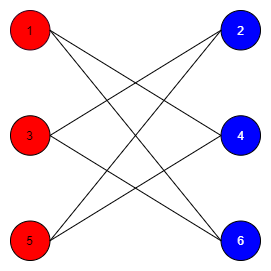
\includegraphics[scale = 0.38]{1a_1}
    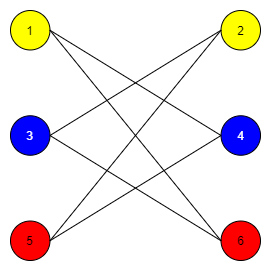
\includegraphics[scale = 0.38]{1a_2}
    \caption{The optimal coloring (left) and the bad coloring (right) of a crown graph with n = 3}
\end{figure}

\pagebreak
\subsection*{b.}
The new greedy algorithm is:
\begin{enumerate}
\item Order the vertices $\{v_1, v_2, ..., v_n\}$ such that $d_{v_{i}} \geq d_{v_{i+1}}$
\item Iterate from 1 to $n$: For each vertice $v_{i}$, give it the smallest possible color.
\end{enumerate}
When the vertex $v_i$ is considered by the algorithm, at most $min(d_{v_i}, i-1)$ of its neighbours have been colored. This is because either all of $v_i$'s neighbours have been colored before $v_i$, or some of them are left untouched, leaving at most $i-1$ neighbours colored. Thus, it would needed at most $min(d_{v_i}, i-1)$ + 1, or $min(d_{v_i} + 1, i)$ colors to color $v_i$ and its previous neighbours (This occurs when all of its neighbours have different colors). And since we are considering the worst case for the algorithm.\\\\
$\Rightarrow$ The maximum number of colors needed by the algorithm is $max_{1 \leq i \leq n}min(d_{i} + 1, i)$.

\pagebreak
\section*{Problem 2}
\subsection*{a.}
\subsection*{The algorithm}
The greedy algorithm for the interval graph coloring is:
\begin{enumerate}
\item Order the nodes $\{v_1, v_2, ..., v_n\}$ such that the starting point of $v_{i}$ is at most the starting point of $v_{i+1}$ (i.e., non decreasing starting point)
\item For each node in the sorted set, give it the smallest possible color.
\end{enumerate}

\subsection*{Proof of correctness}
Let $k$ be the maximum number of intervals intersect each other simultaneously. This means that there will be an edge between every pair of those $k$ nodes. Thus the chromatic number of the graph is at least $k$. The proof is complete if we can show that the algorithm uses at most $k$ colors. \\\\
Assume that the algorithm uses more than $k$ colors. Consider the first time it uses the $k+1^{th}$ color on the node $v_{j}$. Since we order the nodes in non decreasing order of starting points, it means that there must be $k$ nodes starting sooner than $v_{j}$ and intersect with each other. This means that at the nodes $v_{j}$, there are $k+1$ nodes intersect with each other. Implying that the chromatic number of the graph is at least $k+1$. This creates a contradiction. \\\\
$\Rightarrow$ The algorithm uses at most k colors. \\\\
$\Rightarrow$ The algorithm yields the optimum coloring.

\pagebreak
\subsection*{b.}
Consider the below path graph. The chromatic number of the graph is two (as shown in the first picture). But if the algorithm chooses such that two end nodes are colored first, it would need three colors to properly color the graph (the color used and the order of coloring is included in the second picture). I also included the intervals representation of the graph below. Thus, the graph is a valid interval graph and the algorithm fails to use the optimal number of colors. \\\\
\begin{figure}[h]
    \centering
    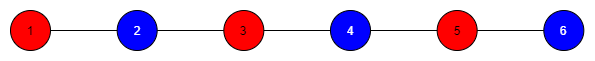
\includegraphics[scale = 0.45]{2b_1}
    \caption{The optimal coloring of a path graph}
\end{figure}
\begin{figure}[h]
    \centering
    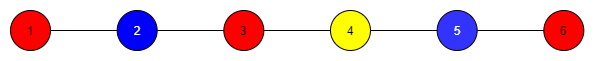
\includegraphics[scale = 0.45]{2b_2}
    \caption{The bad coloring of the path graph, the coloring order is 1 $\rightarrow$ 6 $\rightarrow$ 2 $\rightarrow$ 5 $\rightarrow$ 3 $\rightarrow$ 4}
\end{figure}
\begin{figure}[h]
    \centering
    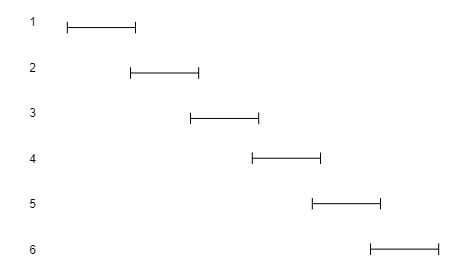
\includegraphics[scale = 0.45]{2b_3}
    \caption{The interval representation of the graph}
\end{figure}

\pagebreak
\section*{Problem 3}
\subsection*{a.}
We can show that the chromatic number of bipartite graphs is two. We can achieve this by coloring the vertices in $B$ with one color, and the vertices in $R$ with another. Since there are no edges between vertices in the same set, the coloring is valid. Thus, the proof is complete if we can show that the algorithm also uses at most two colors. \\\\
To proof this, we can show that the algorithm always color vertices in one set with one color, and vertices in the other set using a different color. We proof this by induction. 
\begin{itemize}
\item Base case: Consider the round after the first color and color degree update. Vertices that are updated must be in the opposite set of the colored vertex (by the bipartite property). Thus, in the next coloring round, one of them will be choose, and colored using a different color with the first vertex.
\item Induction hypothesis: Assume that in the iteration $i$ of color and updat, the colored vertices in the set $B$ all have the same color, and the colored vertices in the set $R$ have another color.
\item Induction: Consider the round $i+1$, let the vertex considered in this round be $v$. Since it is chosen, it means that $v$ must have at least one neighbour that are colored. And by the bipartite property and the hypothesis, all of its neighbour will be in a different set from $v$ and they have the same color. Also, there are no edges between $v$ and any vertices in the same set as $v$. Thus, $v$ must have the same color with vertices that are in the same set with $v$ to maintain a valid coloring. The hypothesis is valid in round $i+1$. 
\end{itemize}
$\Rightarrow$ The algorithm uses two colors, hence it gives the optimum coloring.

\pagebreak
\subsection*{b.}
Consider the graph below. We can easily verify the chromatic number of the graph is 3 (it has odd cycles and can be colored with 3 colors, see the picture for the coloring).
\begin{figure}[h]
    \centering
    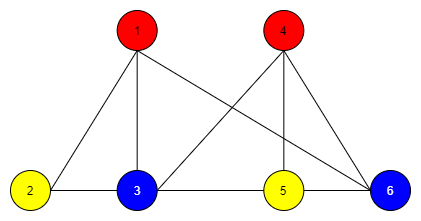
\includegraphics[scale = 0.45]{3b_1}
    \caption{The graph with optimum coloring}
\end{figure} \\
Now, consider the next picture. If we apply the algorithm in the order 1 $\rightarrow$ 2 $\rightarrow$ 3 $\rightarrow$ 6 $\rightarrow$ 4 $\rightarrow$ 5, we get the below coloring. In more details:
\begin{itemize}
\item When vertex 1 is colored red, the color degree of vertices 2, 3, and 6 are updated to 1. We can choose one of them to color next. Choose 2.
\item When vertex 2 is colored blue, the color degree of vertex 3 is updated to 2. Hence the next vertex to be colored must be 3.
\item When vertex 3 is colored yellow, the color degree of vertices 4 and 5 are updated to 1. We can choose one of the vertices 4, 5, and 6 to color next. Choose 6.
\item When vertex 6 is colored blue, the color degree of vertices 4 and 5 are updated to 2. We can choose either of them to color next. Choose 4.
\item When vertex 4 is colored red, vertex 5 is left. Also, since all of 5's neighbours have different colors, it must assume a new color.
\end{itemize}
\begin{figure}[h]
    \centering
    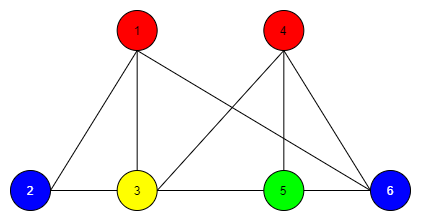
\includegraphics[scale = 0.45]{3b_2}
    \caption{The graph with bad coloring}
\end{figure}
$\Rightarrow$ This example shows that the algorithm is not optimal for general graphs.
 






\end{document}